
\chapter{相关研究综述}
\label{chap:relatedwork}
流行度预测问题自被提出以来,受到了学术界和产业界的广泛关注。本章从流行度的统计特征分析、流行度预测方法以及流行度预测问题的可预测性三个方面入手,对流行度预测领域的相关工作进行了系统的总结和归纳,以便读者更好地了解和掌握该领域的相关知识,进而更好地理解本文的工作。

\section{流行度的统计特征分析}
在线内容的流行度分析工作最早源于网站缓存策略的研究。Cunha等人\citep{chen2005zhulu}在研究站点中网页的访问情况时发现,网页被访问频率的分布服从Zipf定律\citep{chen2005zhulu},也就是说:流行度排名为$i$的网页被用户访问的概率正比于$1/i$,如图\ref{fig:pageDist}所示。这一现象表明,网页的访问频次分布是不均匀的。Almeida等人\citep{chen2005zhulu}在研究万维网中所有网页的访问频次时,也发现了同样的分布规律。
\begin{figure}[!htbp]
  \centering
  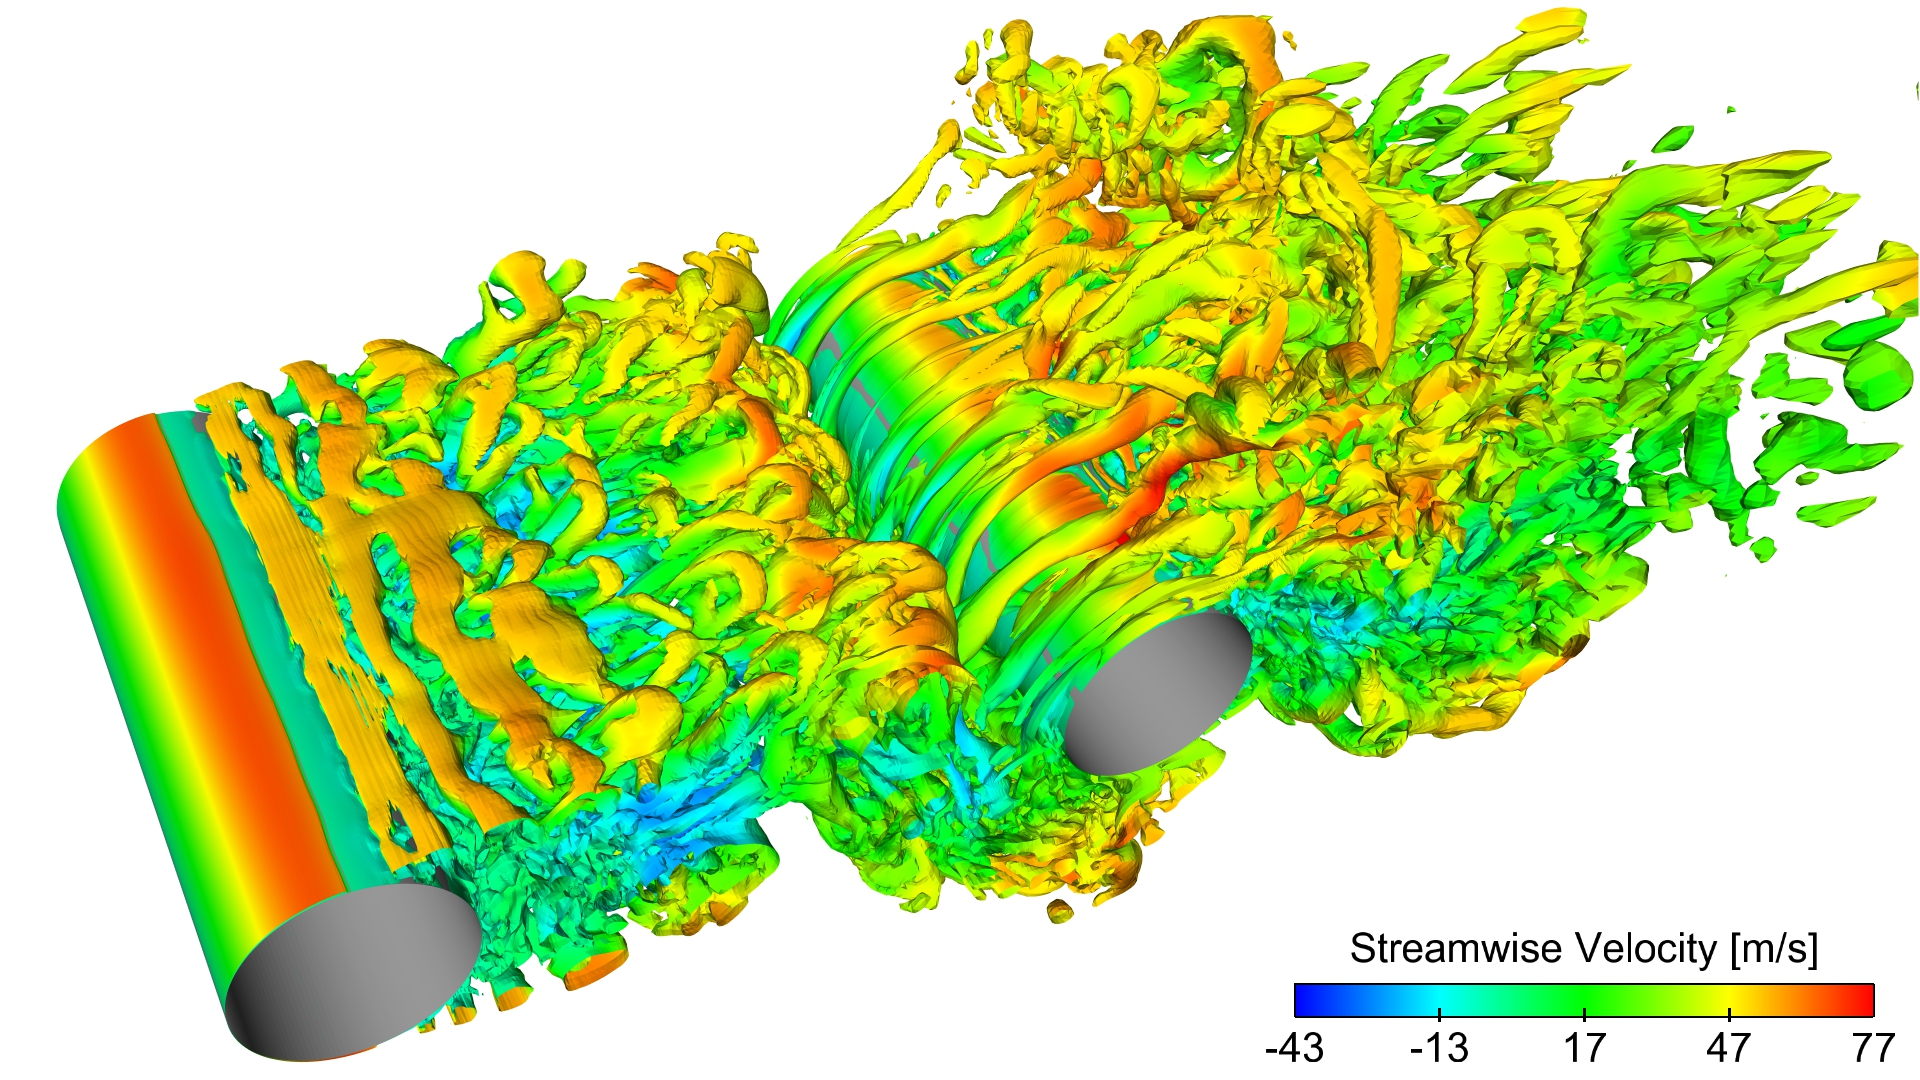
\includegraphics[width=0.45\textwidth]{ITC_Q_Criteria}
  \caption{Q判据等值面图}
  \label{fig:pageDist}
\end{figure}

随着信息技术的发展,视频分享类网站和社交网络平台不断涌现,也引起了研究人员的关注。Gill等人\citep{chen2005zhulu}收集并分析了视频网站Youtube\footnote{\url{https://www.youtube.com}}上视频的访问数据,发现视频的访问频次信息依然服从Zipf定律。Cha等人\citep{chen2005zhulu}对Youtube网站上的视频数据进行了详细的分析,发现网站中不同类别下的视频的观看数分布都服从幂律分布。Kwak等人\citep{chen2005zhulu}研究了社交网络平台Twitter\footnote{\url{https://twitter.com}}上消息的转发情况,发现参与消息转发的人数服从幂律分布,如图\ref{fig:tweetDist}所示。
\begin{figure}[!htbp]
  \centering
  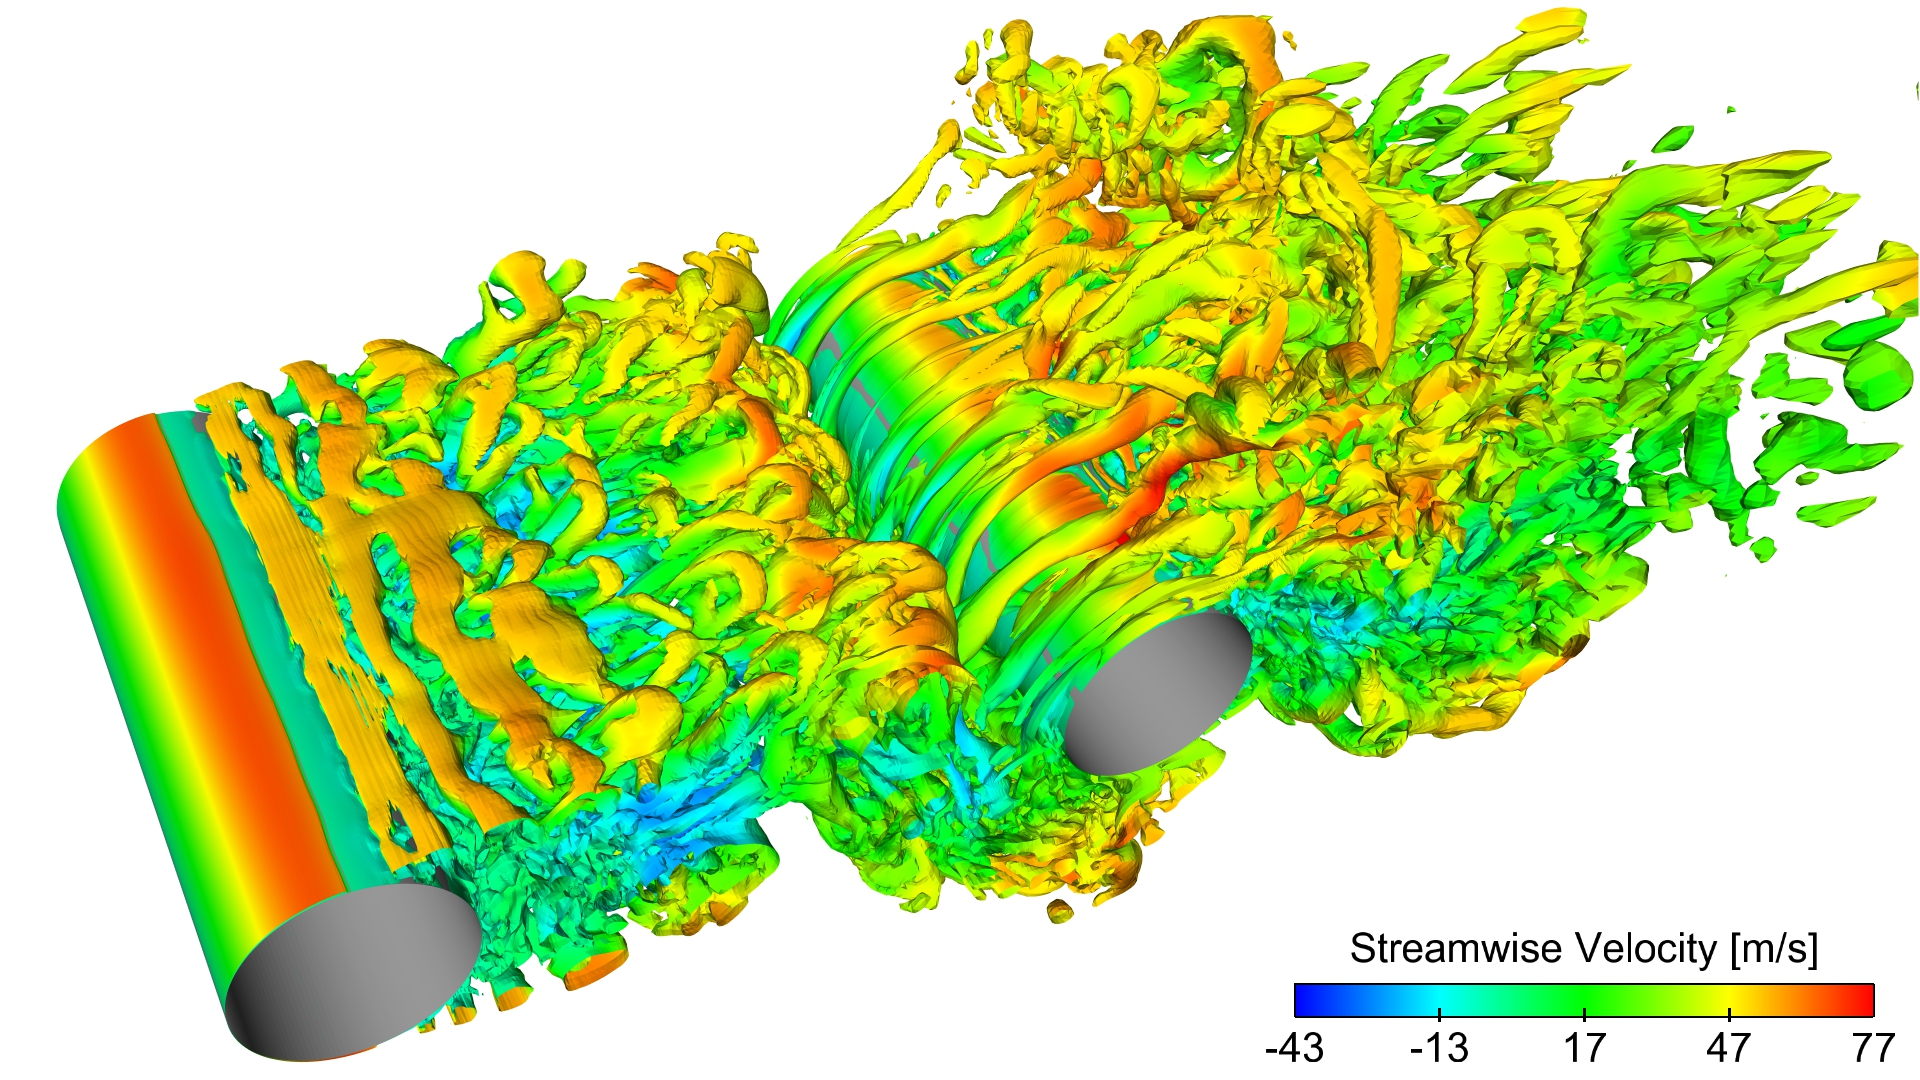
\includegraphics[width=0.45\textwidth]{ITC_Q_Criteria}
  \caption{Q判据等值面图}
  \label{fig:tweetDist}
\end{figure}

除了对宏观的流行度统计量的分析之外,还有一部分工作研究了流行度增长过程中的微观统计特征。Barabasi等人\citep{chen2005zhulu}研究了人类的行为数据,发现人类的行为模式并不是服从传统方法中假设的泊松过程,而是存在爆发现象,并提出了一种基于事件优先级的排队模型来解释这一现象。爆发现象是指人类在参与某类事件时,大部分时间都处于沉寂状态,不会采取任何行为动作;中间夹杂了少数爆发区域,在爆发区域内会有大量的行为数据产生,如图\ref{fig:burst}所示。

爆发现象在在线内容的流行度增长过程中十分常见。Kaltenbrunner等人\citep{chen2005zhulu}研究了新闻评论网站Slashdot\footnote{\url{https://slashdot.org}}上新闻的评论情况,并对评论数据的时间间隔分布进行了分析。统计结果表明,评论数据的时间间隔分布是两个log-normal分布的混合,并且存在明显的周期现象。Bao等人\citep{chen2005zhulu}研究了新浪微博中消息的转发时间间隔数据,发现转发时间间隔分布服从幂律分布,这也说明了社交网络中消息的流行度累积过程中存在爆发现象。
\begin{figure}[!htbp]
  \centering
  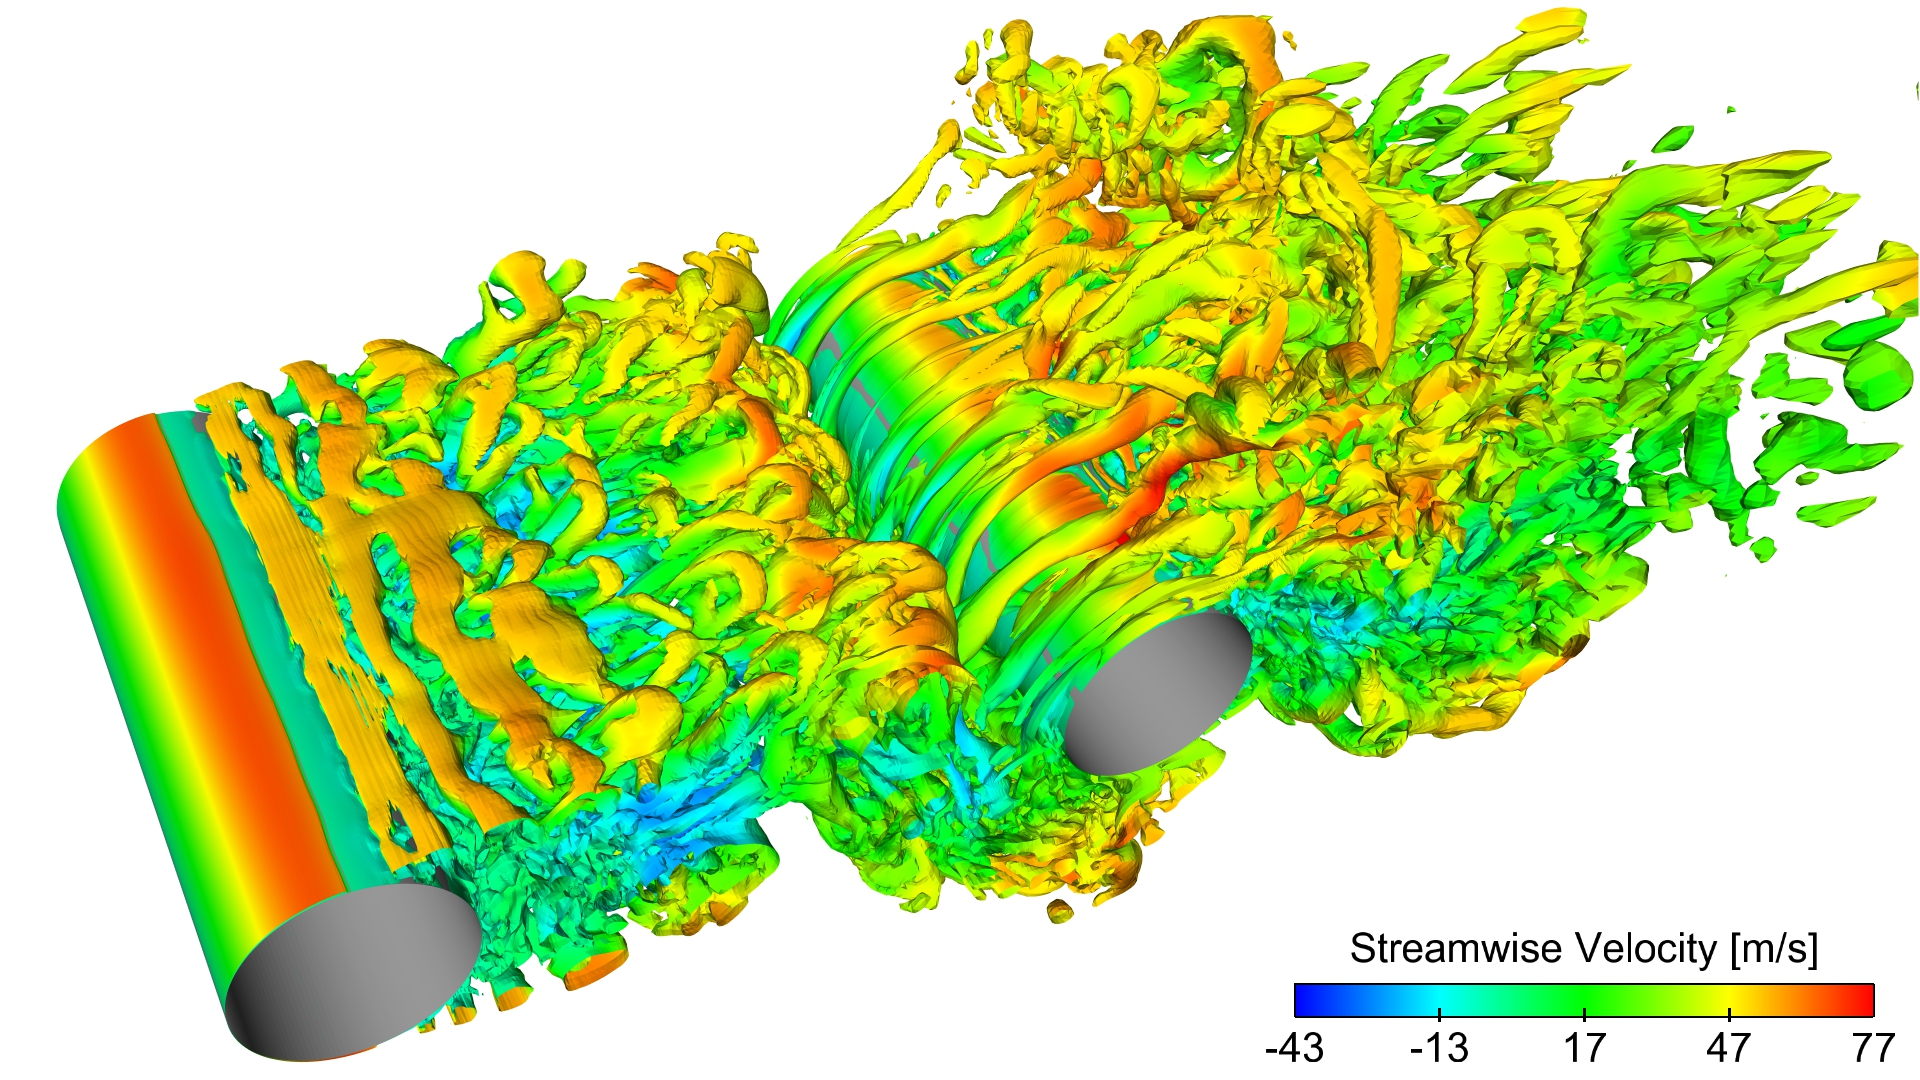
\includegraphics[width=0.45\textwidth]{ITC_Q_Criteria}
  \caption{Q判据等值面图}
  \label{fig:burst}
\end{figure}

除爆发现象外,研究人员还发现流行度的增长过程中存在着固定的模式。Yang等人\citep{chen2005zhulu}研究了Twitter平台上消息的传播过程,提出了K-SC(K-Spectral Centroid)聚类方法,对消息的流行度变化过程进行聚类,将消息的流行度变化过程聚为六类,如图\ref{fig:pattern}所示。此外,Costa等人\citep{chen2005zhulu}还发现流行度的增长过程中呈现出明显的周期性特点。
\begin{figure}[!htbp]
  \centering
  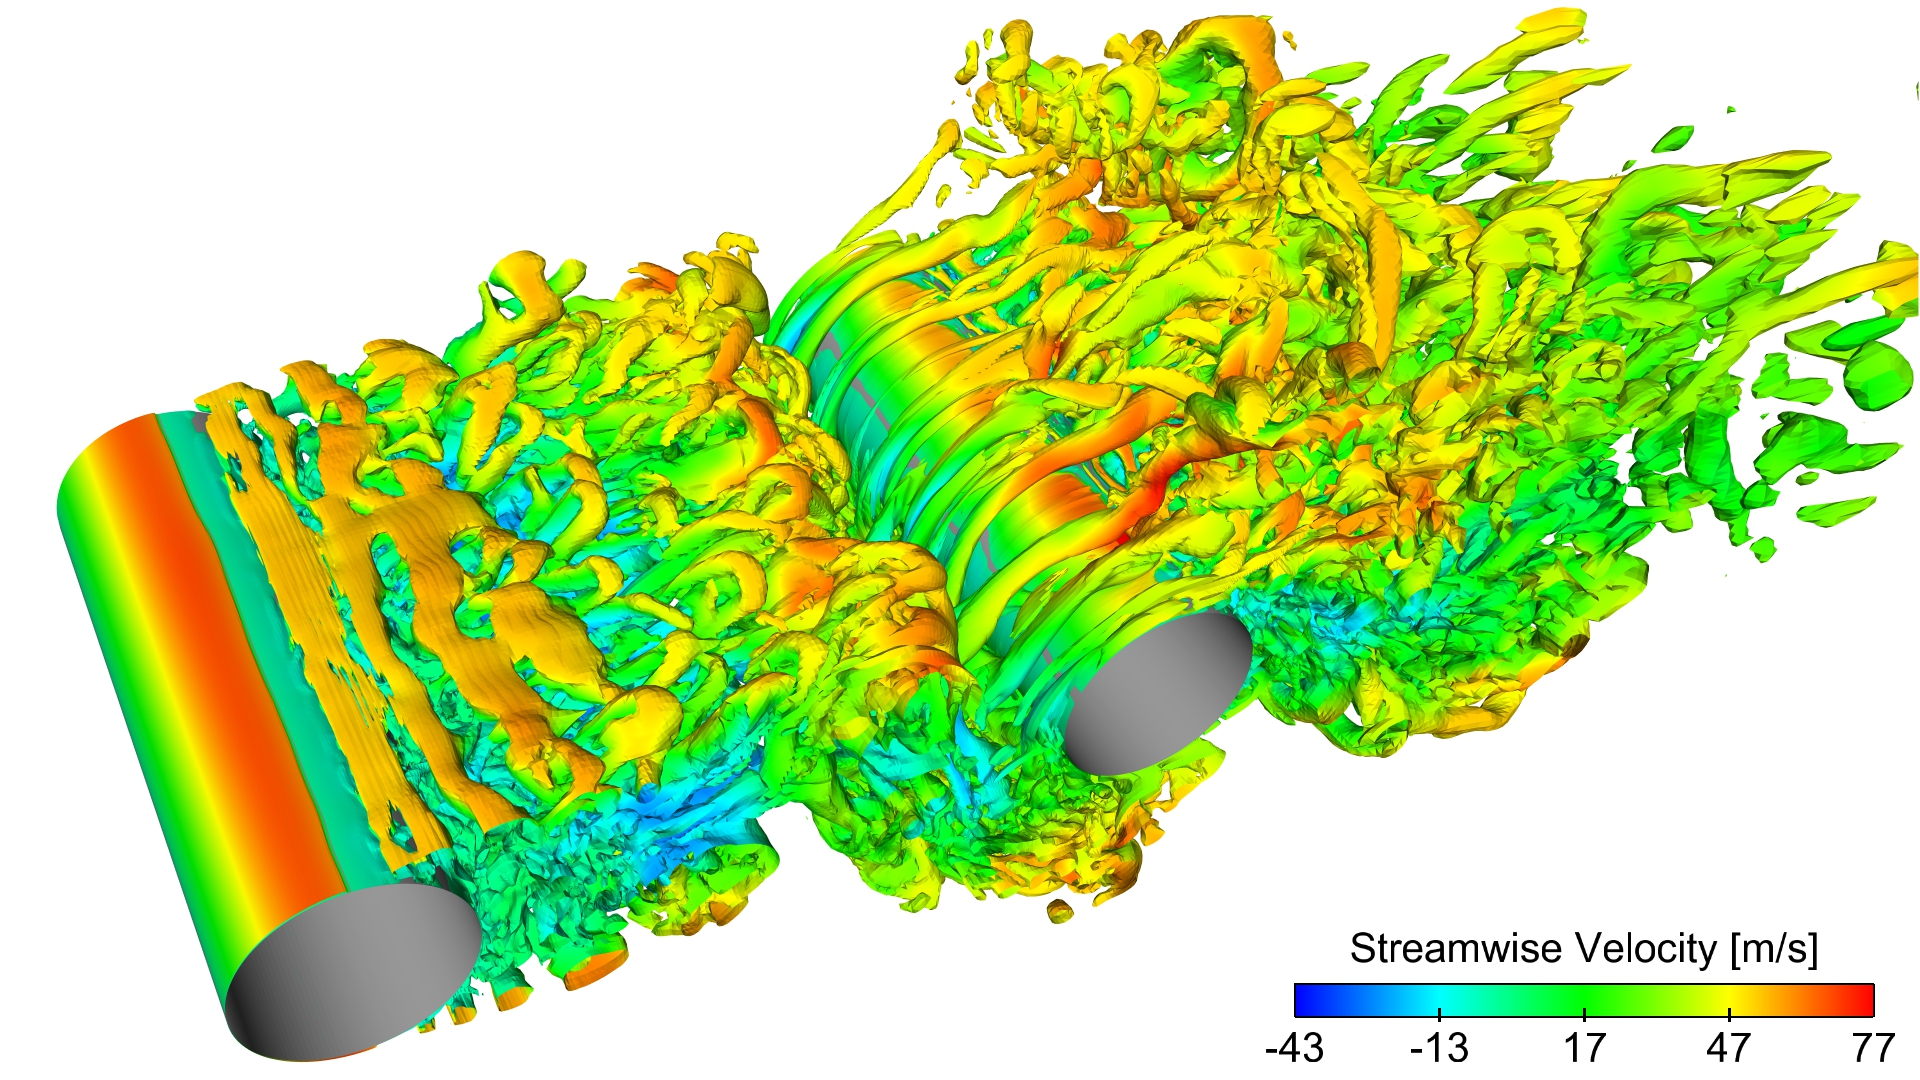
\includegraphics[width=0.45\textwidth]{ITC_Q_Criteria}
  \caption{Q判据等值面图}
  \label{fig:pattern}
\end{figure}

流行度分布的不均匀性,以及增长过程出现的爆发现象和时序特性,吸引了大量研究人员的关注,进而涌现出了多种流行度预测的模型和方法。
\section{流行度预测方法概述}
现有的流行度预测方法主要包含三类:基于特征的有监督学习方法、基于点过程的流行度到达过程建模方法和基于表示学习的方法。本节会依次对这三类方法进行介绍和总结。
\subsection{基于特征的有监督学习方法}
基于特征的流行度预测方法主要通过借助已有的有监督学习模型,结合人工抽取的特征,来对流行度的增长过程进行预测。在这类方法中,流行度预测问题通常会被形式化为分类或者回归问题。Cha等人\citep{chen2005zhulu}分析了Youtube网站上视频的流行度增长数据,发现视频上传7天后的访问量和视频上传后一天以及上传后两天的访问量之间存在着非常强的相关性,进而提出了预测视频近期流行度的任务。Szabo等人\citep{chen2005zhulu}研究了Digg\footnote{\url{http://digg.com}}网站上的新闻数据和Youtube网站上的视频数据,发现这些内容早期的流行度和后期的流行度在进行对数变换后,存在着非常强的线性相关性,如图\ref{fig:loglinear}所示。基于这一观测,他们提出了S-H(Szabo-Huberman)模型,
\begin{figure}[!htbp]
  \centering
  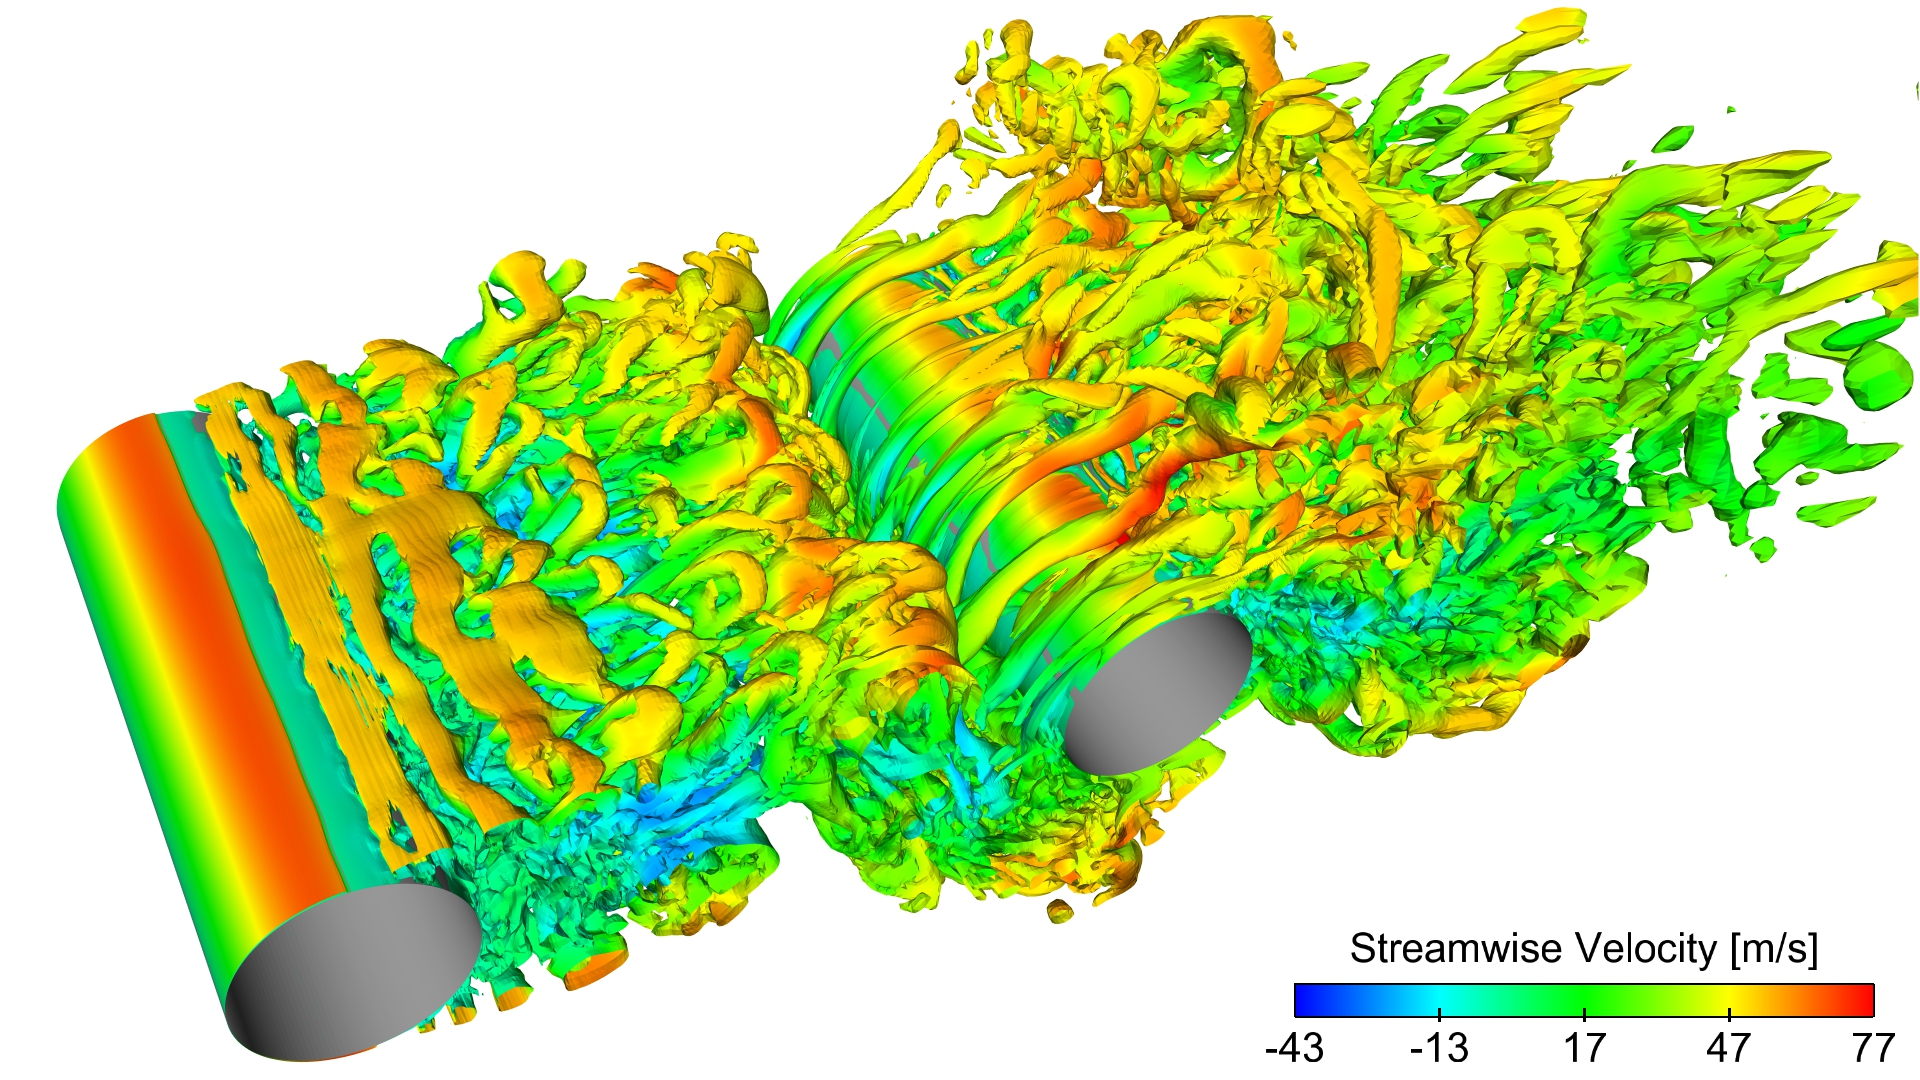
\includegraphics[width=0.45\textwidth]{ITC_Q_Criteria}
  \caption{Q判据等值面图}
  \label{fig:loglinear}
\end{figure}

\subsection{基于点过程的流行度到达过程建模方法}
\subsection{基于表示学习的方法}
\subsection{其他方法}
\section{流行度预测问题的可预测性分析}

